\chapter{Architectural design} \label{chap:architectural}


\section{Overview}
This chapter, arguably the longest of this document, analyses all the different aspects of the architecture of myTaxiService system, at different levels of detail and from different points of view.

In \cref{sec:highlevel} we give a high level description of the structure of the system. Inevitably this section will be pretty abstract.

Then, \cref{sec:componentView} focuses on the components of the system. With the word \emph{component} we refer to an independent software element that encapsulates a set of related functions. This is to say that a component is defined by its interfaces. The interfaces between the components are fully analysed in \cref{sec:componentInterfaces}. In opposition to the focus on the interactions within the system, the deployment view in \cref{sec:deployment} provides further details on the physical structure of its various parts.

In the runtime view (\cref{sec:runtime}) we show the behaviour of the system in case of a request and a reservation. 

Finally, \cref{sec:styles} is meant to give further details and explanations about our design and architectural choices. 

UML being an agreed and relatively easy to understand language, in the whole chapter we will make extensive use of it.


\section{High level components and their interaction}\label{sec:highlevel}
For our myTaxiService ecosystem, we will adopt the Java Enterprise Edition\footnote{In the following, simply JavaEE.} application model for enterprise applications. This will allow the design, building and production of a solid, fast and reliable system, with a special focus on money and resources. We believe that such an architecture can be easy to understand and to set up; also, it is highly scalable, which is a huge bonus since we cannot foresee the evolution of the use of the system in the city.

\begin{figure}%
	\centering%
	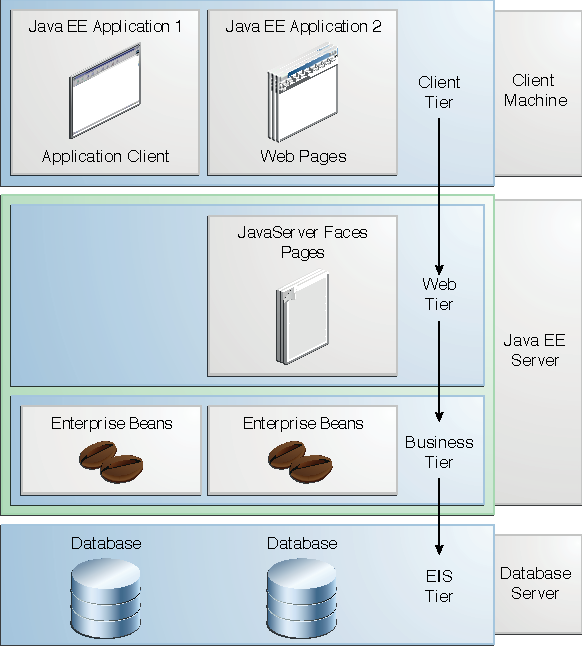
\includegraphics[width=0.83\textwidth]{img/JEETT}%
	\caption{High level architecture. Source: \emph{Java Platform, Enterprise Edition. The Java EE Tutorial, Release 7}. Oracle, September 2014.}\label{fig:jeett}%
\end{figure}

The JavaEE platform uses a distributed multitiered application model. Application logic is divided into components according to function, and the application components that make up a JavaEE application are installed on various machines depending on the tier to which the application component belongs. \Cref{fig:jeett} shows the model we will adopt, which consists of four tiers:

\begin{description}
	\item [Client tier] it contains all the components which run on the client machine (applications, web pages); in our case myTaxiWeb web pages, and myTaxiApp, myTaxiAssist mobile applications are the clients. These all are \emph{thin clients}, which means that they do not directly query the database, nor execute complex operations. 
	
	\item [Web tier] the components of this tier run on the JavaEE server; this tier is intended to manage the data flow between clients and JavaEE.

	\item [Business tier] this tier, which runs on the JavaEE server as well, contains the so called \emph{enterprise beans}. Enterprise beans handle business code, which is logic that govern myTaxiService system; to do so, they also retrieve data from storage, processes it (if necessary), and sends it back to the client program, through the web tier.

	\item [EIS tier] this tier, typically, handles EIS\footnote{EIS stands for Enterprise information system.} software and includes enterprise infrastructure systems, such as enterprise resource planning (ERP), mainframe transaction processing, database systems, and other legacy information systems. In our specific context, JavaEE application components might need access to enterprise information systems for database connectivity.
	
\end{description}


\section{Component view}\label{sec:componentView}
Now let us refine what was given in \cref{sec:highlevel}. In the following component diagram (\cref{fig:component}) the architecture of the system has been expanded.

\begin{figure*}%
	\centering%
	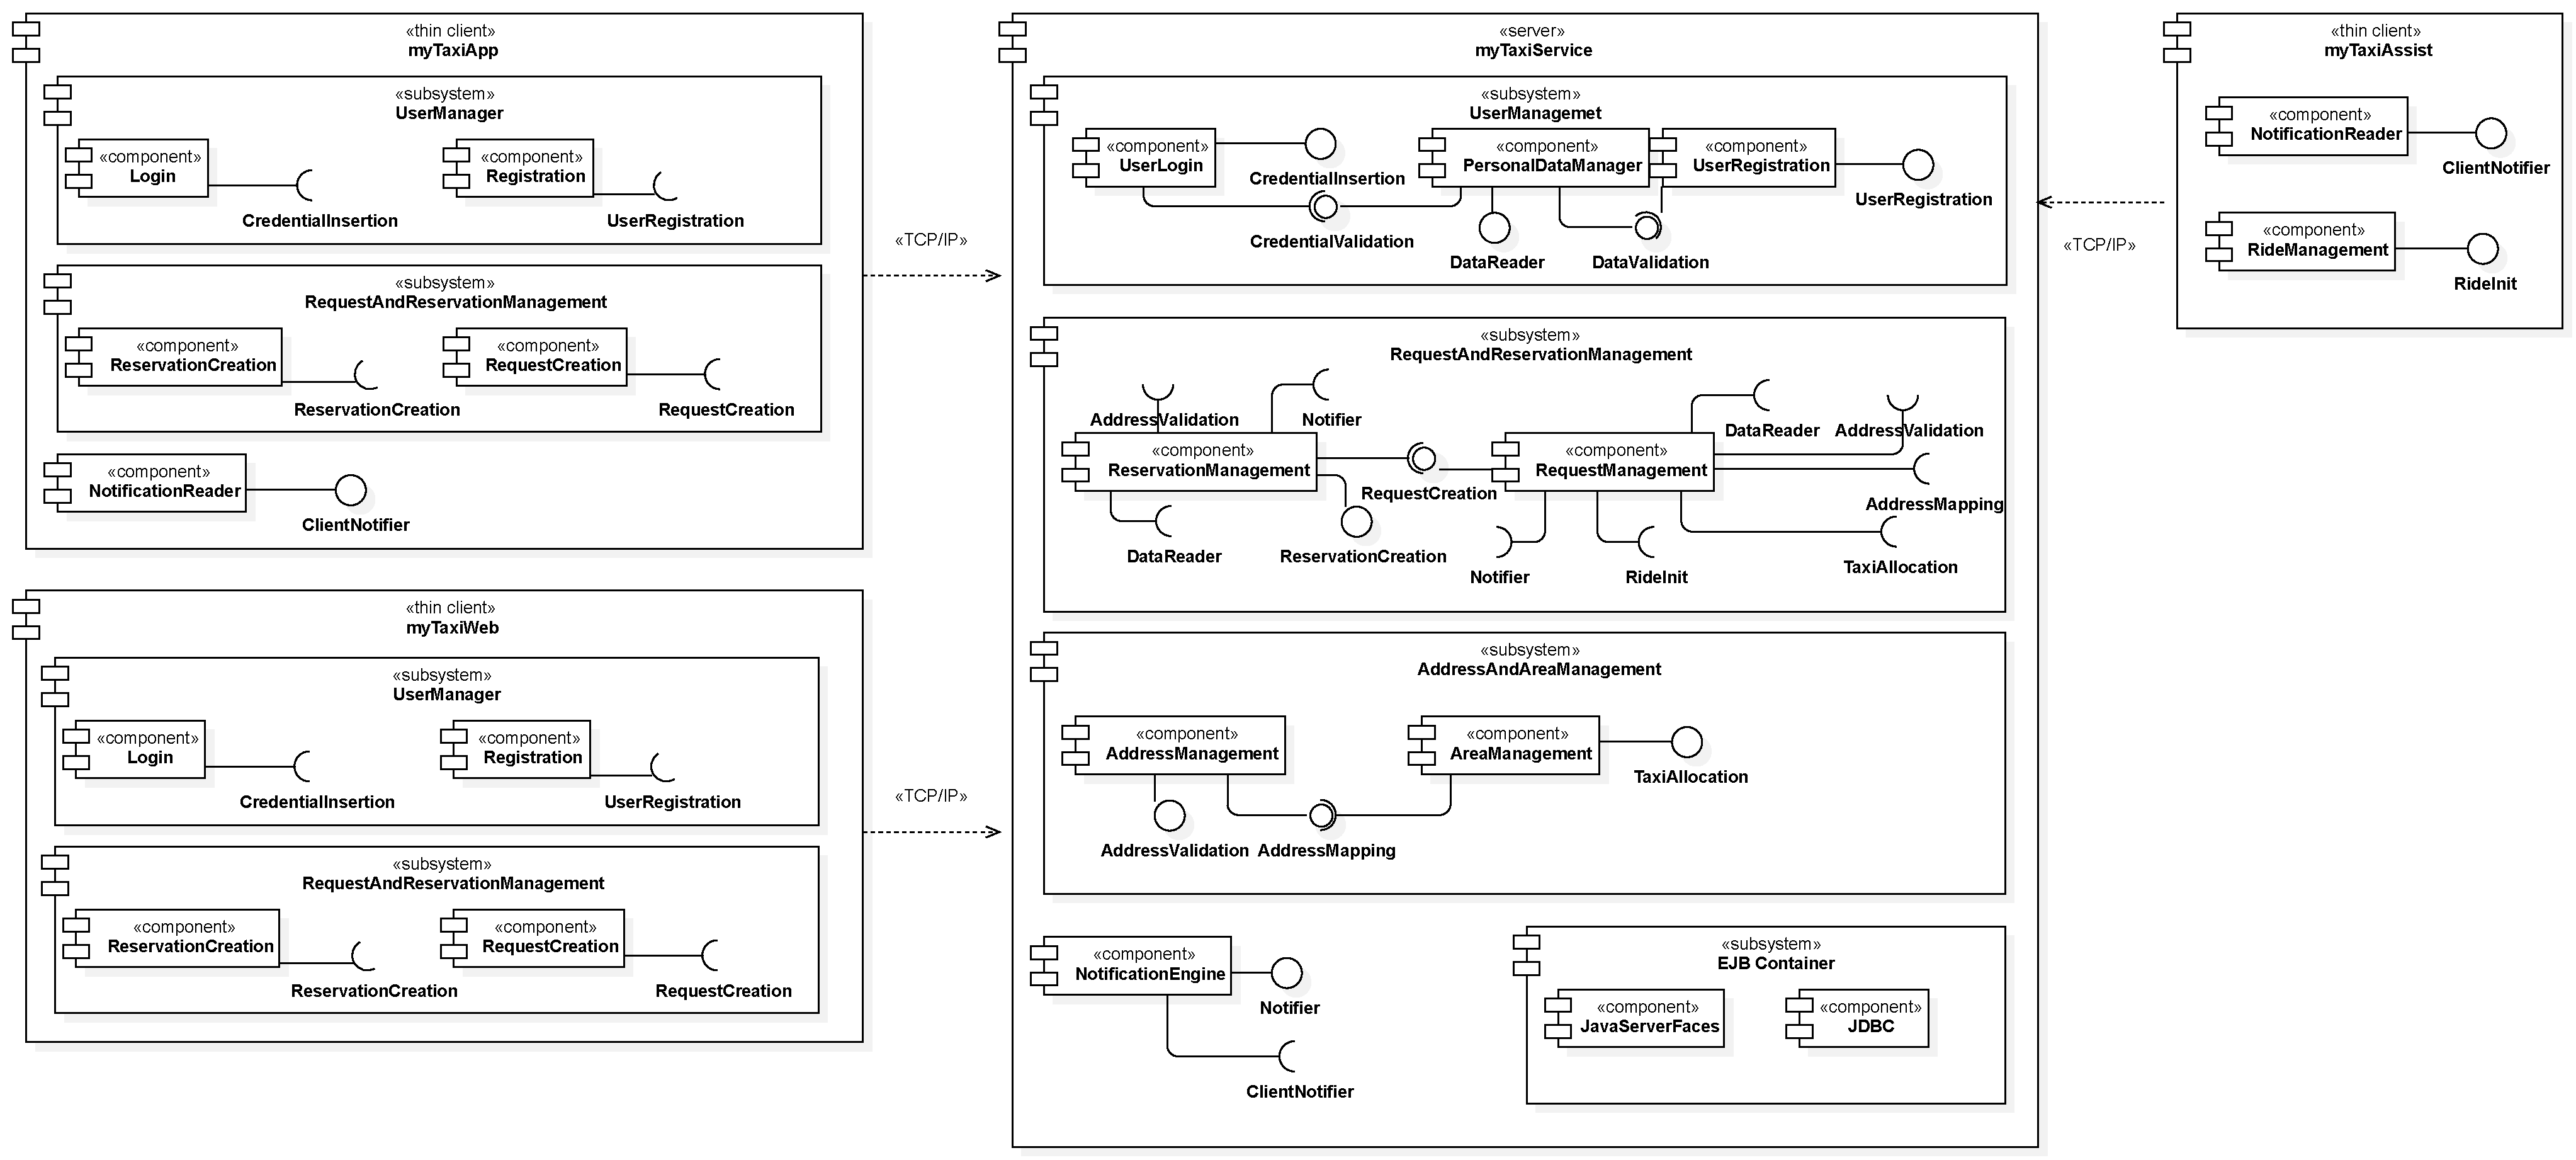
\includegraphics[width=\textwidth]{img/ComponentView__ComponentDiagram_1}%
	\caption{Component diagram.}\label{fig:component}%
\end{figure*}

In the diagram, each application of the system (myTaxiApp, myTaxiWeb, myTaxiAssist, myTaxiService) is represented, together with its own components. Moreover, for the sake of clarity, some subsystems have been introduced, to gather logically similar components. Each component may offer or require some interfaces. These interfaces reflect the services that the component provides (which are indicated in UML by a circle at the end of a line from the component icon) and the services that the component requires to operate correctly (the symbol for this kind of interface is a semicircle at the end of a line from the component icon).

For example, let us consider the \texttt{Re\-quest\-And\-Res\-er\-va\-tion\-Man\-age\-ment} subsystem in myTaxiService server. It has two components, \texttt{Res\-er\-va\-tion\-Man\-age\-ment} and \texttt{Re\-quest\-Man\-age\-ment}. The former, as the name suggests, handles the reservations, from the reception until their conversion to requests\footnote{\label[sidenote]{foot:reservConversion}Remember that our system confirms the reservation and allocates a taxi \num{10} minutes before the meeting time with the customer, as though it was a request.}. In order to do the conversion, the component needs a service, namely \texttt{Re\-quest\-Cre\-ation}, which is conveniently offered by \texttt{Re\-quest\-Man\-age\-ment} component.

For the sake of clarity, we preferred to draw only the connections between the applications, and to exclude all the links between interfaces that would lie outside the subsystems. By doing so, we avoid the otherwise inevitable tangle of connections. Correspondence is given by giving the same name to offered and required services; however, further details about the interfaces are provided in \cref{sec:componentInterfaces}.

Before we proceed with our analysis, we would like to focus our attention on two components in myTaxiService server, \texttt{Java\-Ser\-ver\-Faces} and \texttt{Java\-Per\-sist\-ence\-API}. They both provide all the JavaBeans components\footnote{\emph{JavaBeans} denotes a set of standards and conventions useful to build components in Java language.} which are essential for the operation of the system. The former handles the server side for the clients, the latter instead makes the usage of MySQL database management system possible.


\section{Component interfaces}\label{sec:componentInterfaces}
In this section we are going to analyse the most significant interfaces between components which were shown in \cref{fig:component}. In the following table, the components are presented along with the interface they offer and a brief description.


%Component - Interfaces provided - Description

\newcommand{\cW}{4cm}
\newcommand{\iW}{3.5cm}

\begin{figure*}\begin{tabularx}{\textwidth}{ >{\bfseries}c C{\iW} X }\toprule%
%
\normalfont{\centering\textsc{Component}} & \normalfont{\centering\textsc{Interfaces}} & \normalfont{\textsc{Description}}
\\%
\toprule%
%
	AddressManagement%
	&% 
	AddressMapping%
	&%
	Provides the methods to map addresses into the system, returning the corresponding area.%
%	
	\\% 
	\cmidrule{2-3}%
%
	&%
	AddressValidation% 
	&%
	Offers the methods to validate addresses, checking their existence in the database. Also converts addresses in GPS coordinates and vice versa.	%
%	
\\% 
\midrule%
%
	AreaManagement% 
	&% 
	TaxiAllocation% 
	&% 
	Provides the methods for managing the taxi allocation (e.g., enqueue and dequeue, and the change of a taxi availability).%
%	
\\% 
\midrule%
%
	NotificationEngine% 
	&% 
	Notifier% 
	&% 
	Provides the methods for the notification of client systems.%
%	
\\% 
\midrule%
%
	NotificationReader% 
	&% 
	ClientNotifier% 
	&% 
	Provides the methods to notify the customers.%
%	
\\% 
\midrule%
%
	PersonalDataManager%
	&% 
	CredentialValidation% 
	&% 
	Provides the methods that check the personal credentials in the database.%
%	
	\\% 
	\cmidrule{2-3}%
%	
	&%
	DataValidation%
	&%
	Provides all the methods to validate personal data, for instance the correctness of the name (it cannot contain numbers) or of a birthdate (it shall not be in the future).%
%	
	\\% 
	\cmidrule{2-3}%
%	
	&%
	DataReader%
	&%
	Offers the methods to access customer data, stored in the database.%
%	
\\% 
\midrule%
%
	RequestManagement% 
	&% 
	RequestCreation% 
	&% 
	Offers the methods to make a request. It validates data, interacts with the required components to allocate a taxi and stores the request in the database.%	
%
\\% 
\midrule%
%
	ReservationManagement% 
	&% 
	ReservationCreation% 
	&% 
	Provides the methods to make a reservation. It interacts with other components for data validation and storing.%
%
\\% 
\midrule%
%
	RideManagement% 
	&% 
	RideInit% 
	&% 
	Provides the methods necessary to instantiate a ride for the driver. This component interacts also with the on board navigator.%
%
%
\\% 
\bottomrule%
\end{tabularx}%
\end{figure*}
\clearpage
\begin{figure*}\begin{tabularx}{\textwidth}{ >{\bfseries}c C{\iW} X }\toprule
\normalfont{\centering\textsc{Component}} & \normalfont{\centering\textsc{Interfaces}} & \normalfont{\textsc{Description}}%
\\%
\toprule%
%	
	UserLogin% 
	&% 
	CredentialInsertion% 
	&% 
	Offers the methods useful to log in a User (both a registered customer and a taxi driver). It interacts with \texttt{Per\-son\-al\-Data\-Man\-ager} component to complete the login and start the user session.%
%	
\\% 
\midrule%
%	
	UserRegistration% 
	&% 
	UserRegistration% 
	&% 
	Provides the methods for the insertion of a new customer in the database, validating his data.%
%	
\\% 
\bottomrule%	
\end{tabularx}%
\end{figure*}

Notice that PersonalDataManager \texttt{Per\-son\-al\-Data\-Man\-ager} component allows access to the personal data, which are stored in the database. Moreover, it provides validation methods on all the personal data.


\section{Deployment view}\label{sec:deployment}
After focusing on the logical structure of the system and on the interactions within, it is appropriate to provide a lower level view on the architecture of the system. In particular the deployment diagram in \cref{fig:deployment} shows the distribution of the concrete software artefacts\footnote{That is, files and libraries.} over the various computational nodes of our system.

\begin{figure*}%
	\centering%
	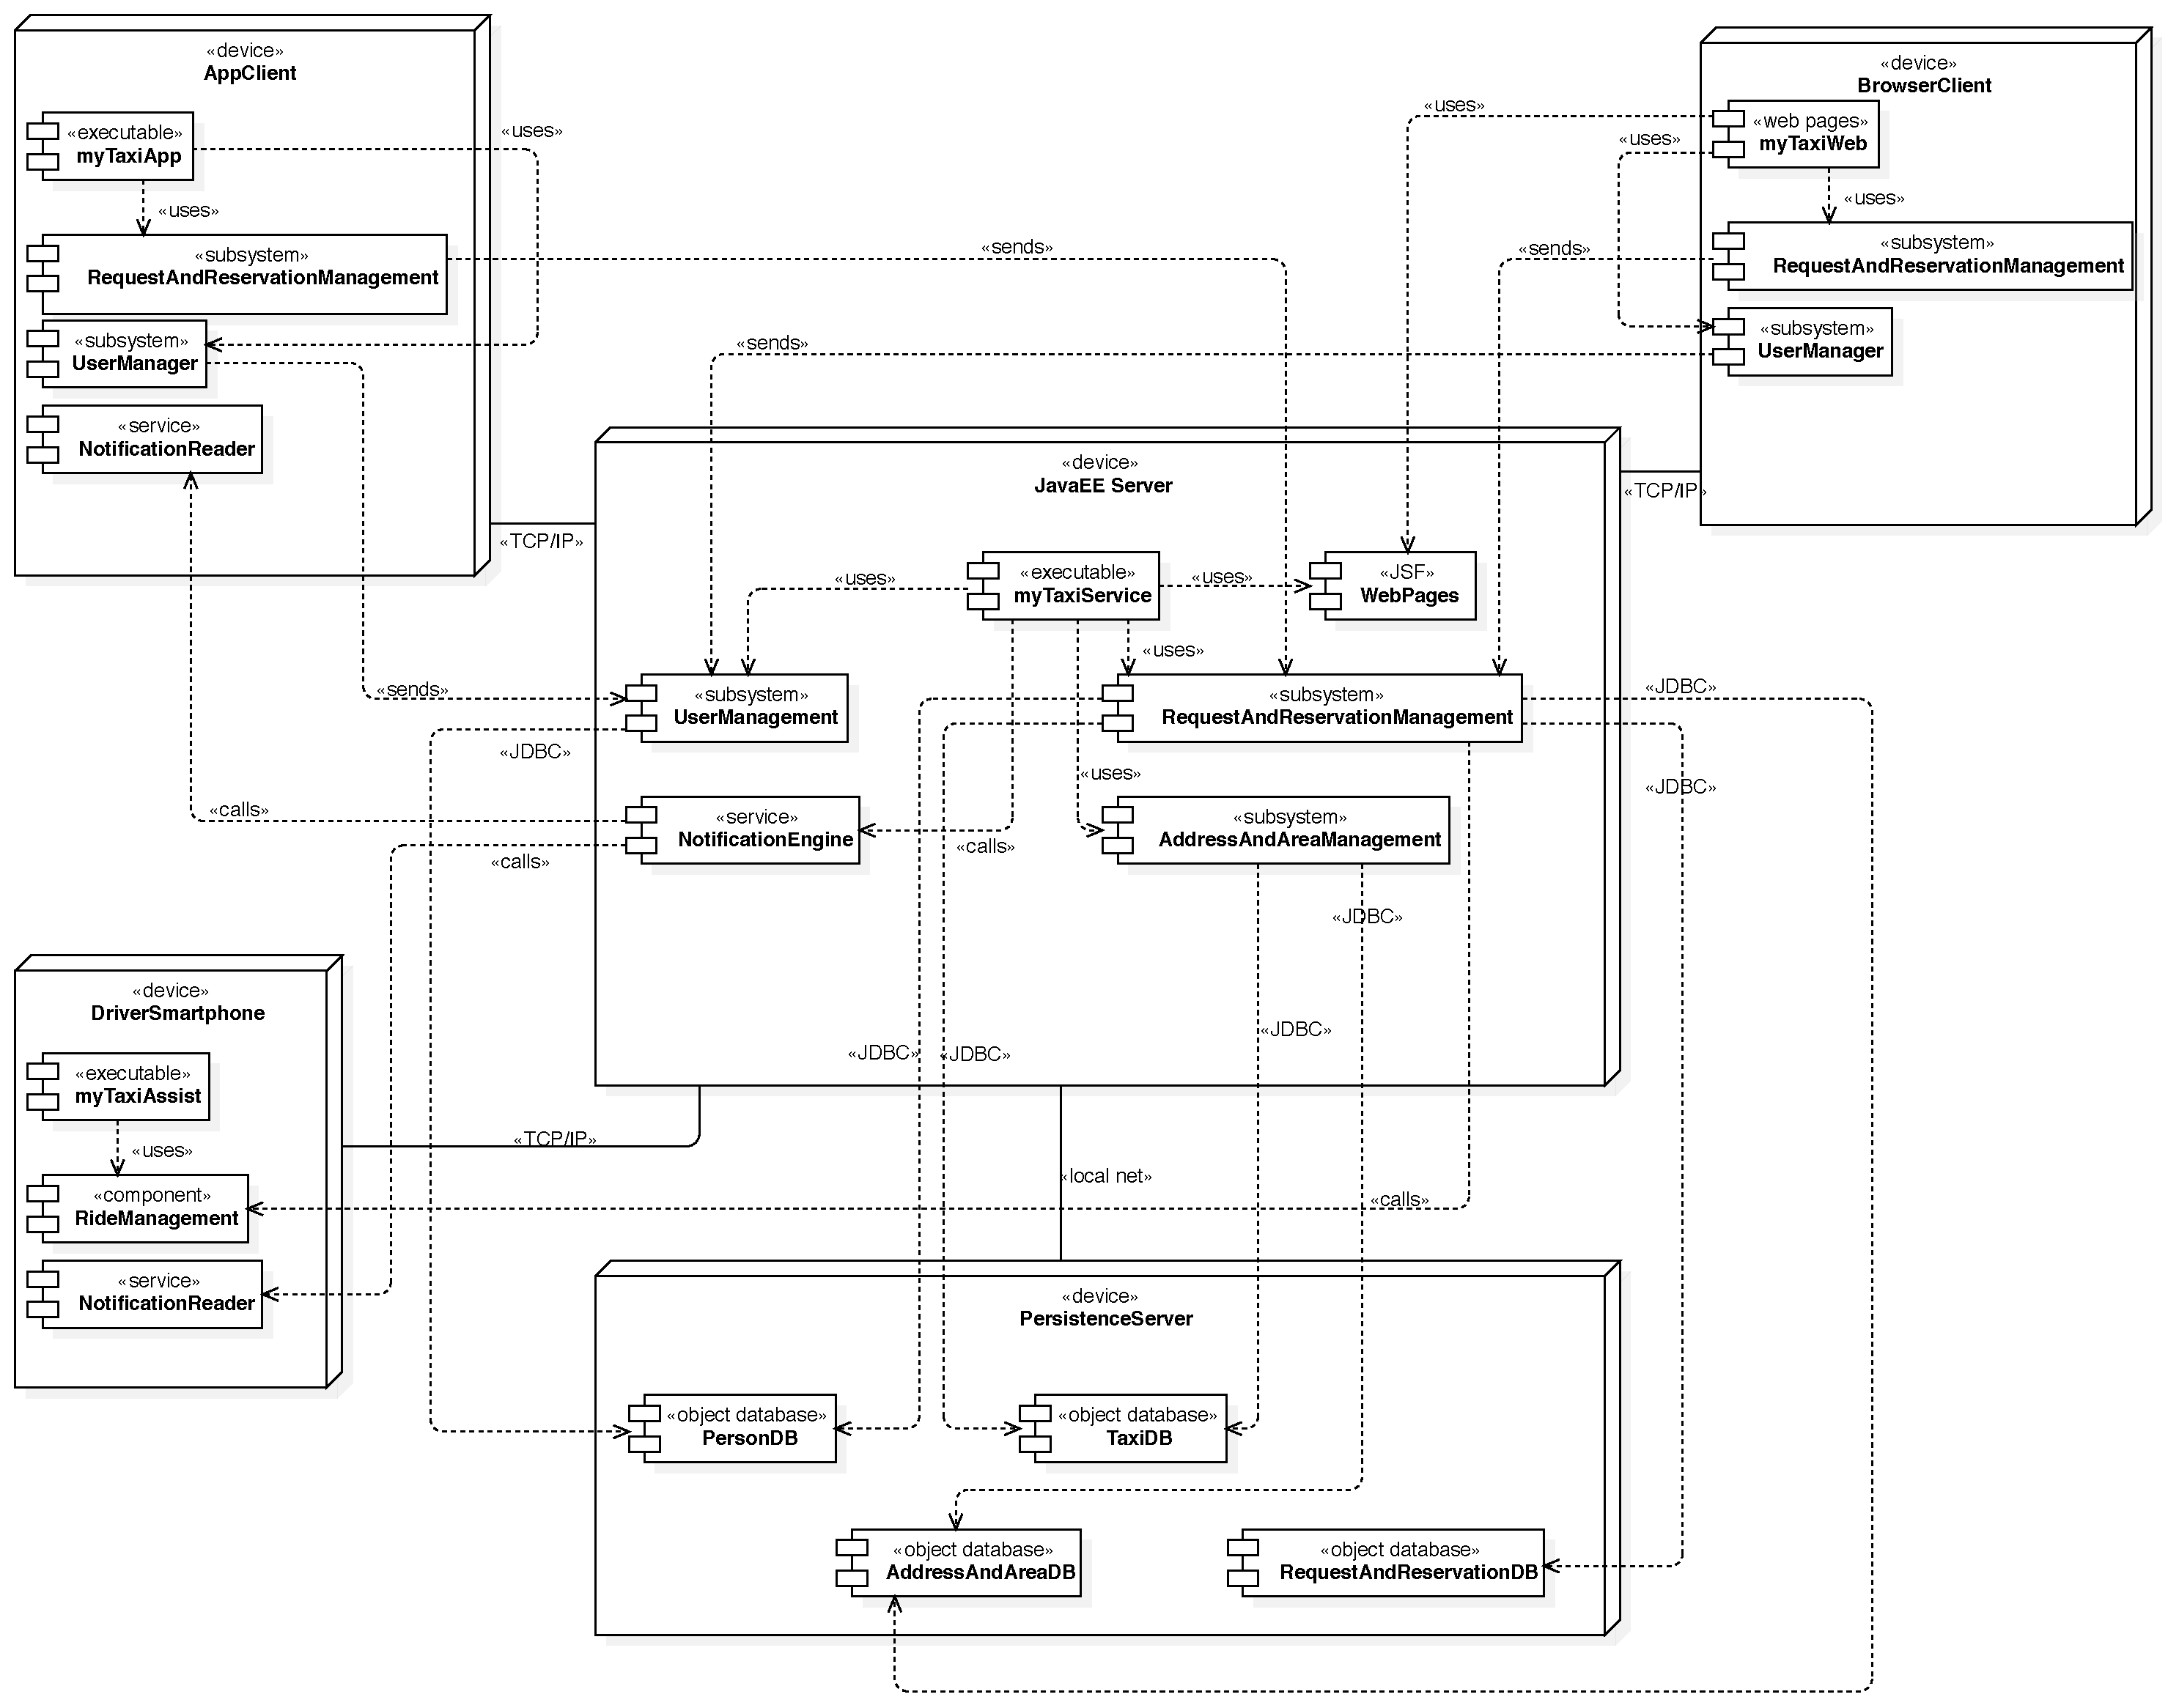
\includegraphics[width=\textwidth]{img/Deploy__DeploymentDiagram_4}%
	\caption{Deployment diagram.}\label{fig:deployment}%
\end{figure*}

To reflect the architecture outlined in \cref{sec:highlevel}, the diagram develops over three types of hardware systems: \texttt{App\-Cli\-ent}, \texttt{Brows\-er\-Cli\-ent} and \texttt{Driver\-Smart\-phone} are the three possible client machines, then we have the \texttt{Java\-EE Ser\-ver}, intended for the business logic, and the \texttt{Per\-sist\-ence\-Ser\-ver}, dedicated to the database.

The main interactions between the components have been drawn. Moreover, the nature of the various components (executable, service) has been specified, so as to give a more complete view on the architecture of the system.



\section{Runtime view}\label{sec:runtime}
Before introducing a runtime view of myTaxiService (\cref{fig:runtime}), we would like to expand the two sequence diagrams which were presented in the \rasd regarding the request and the reservation of a taxi ride (in that document they are, respectively, figure~3.2 and figure~3.10) in order to show the actual behaviour of the system.

\begin{figure*}%
	\centering%
	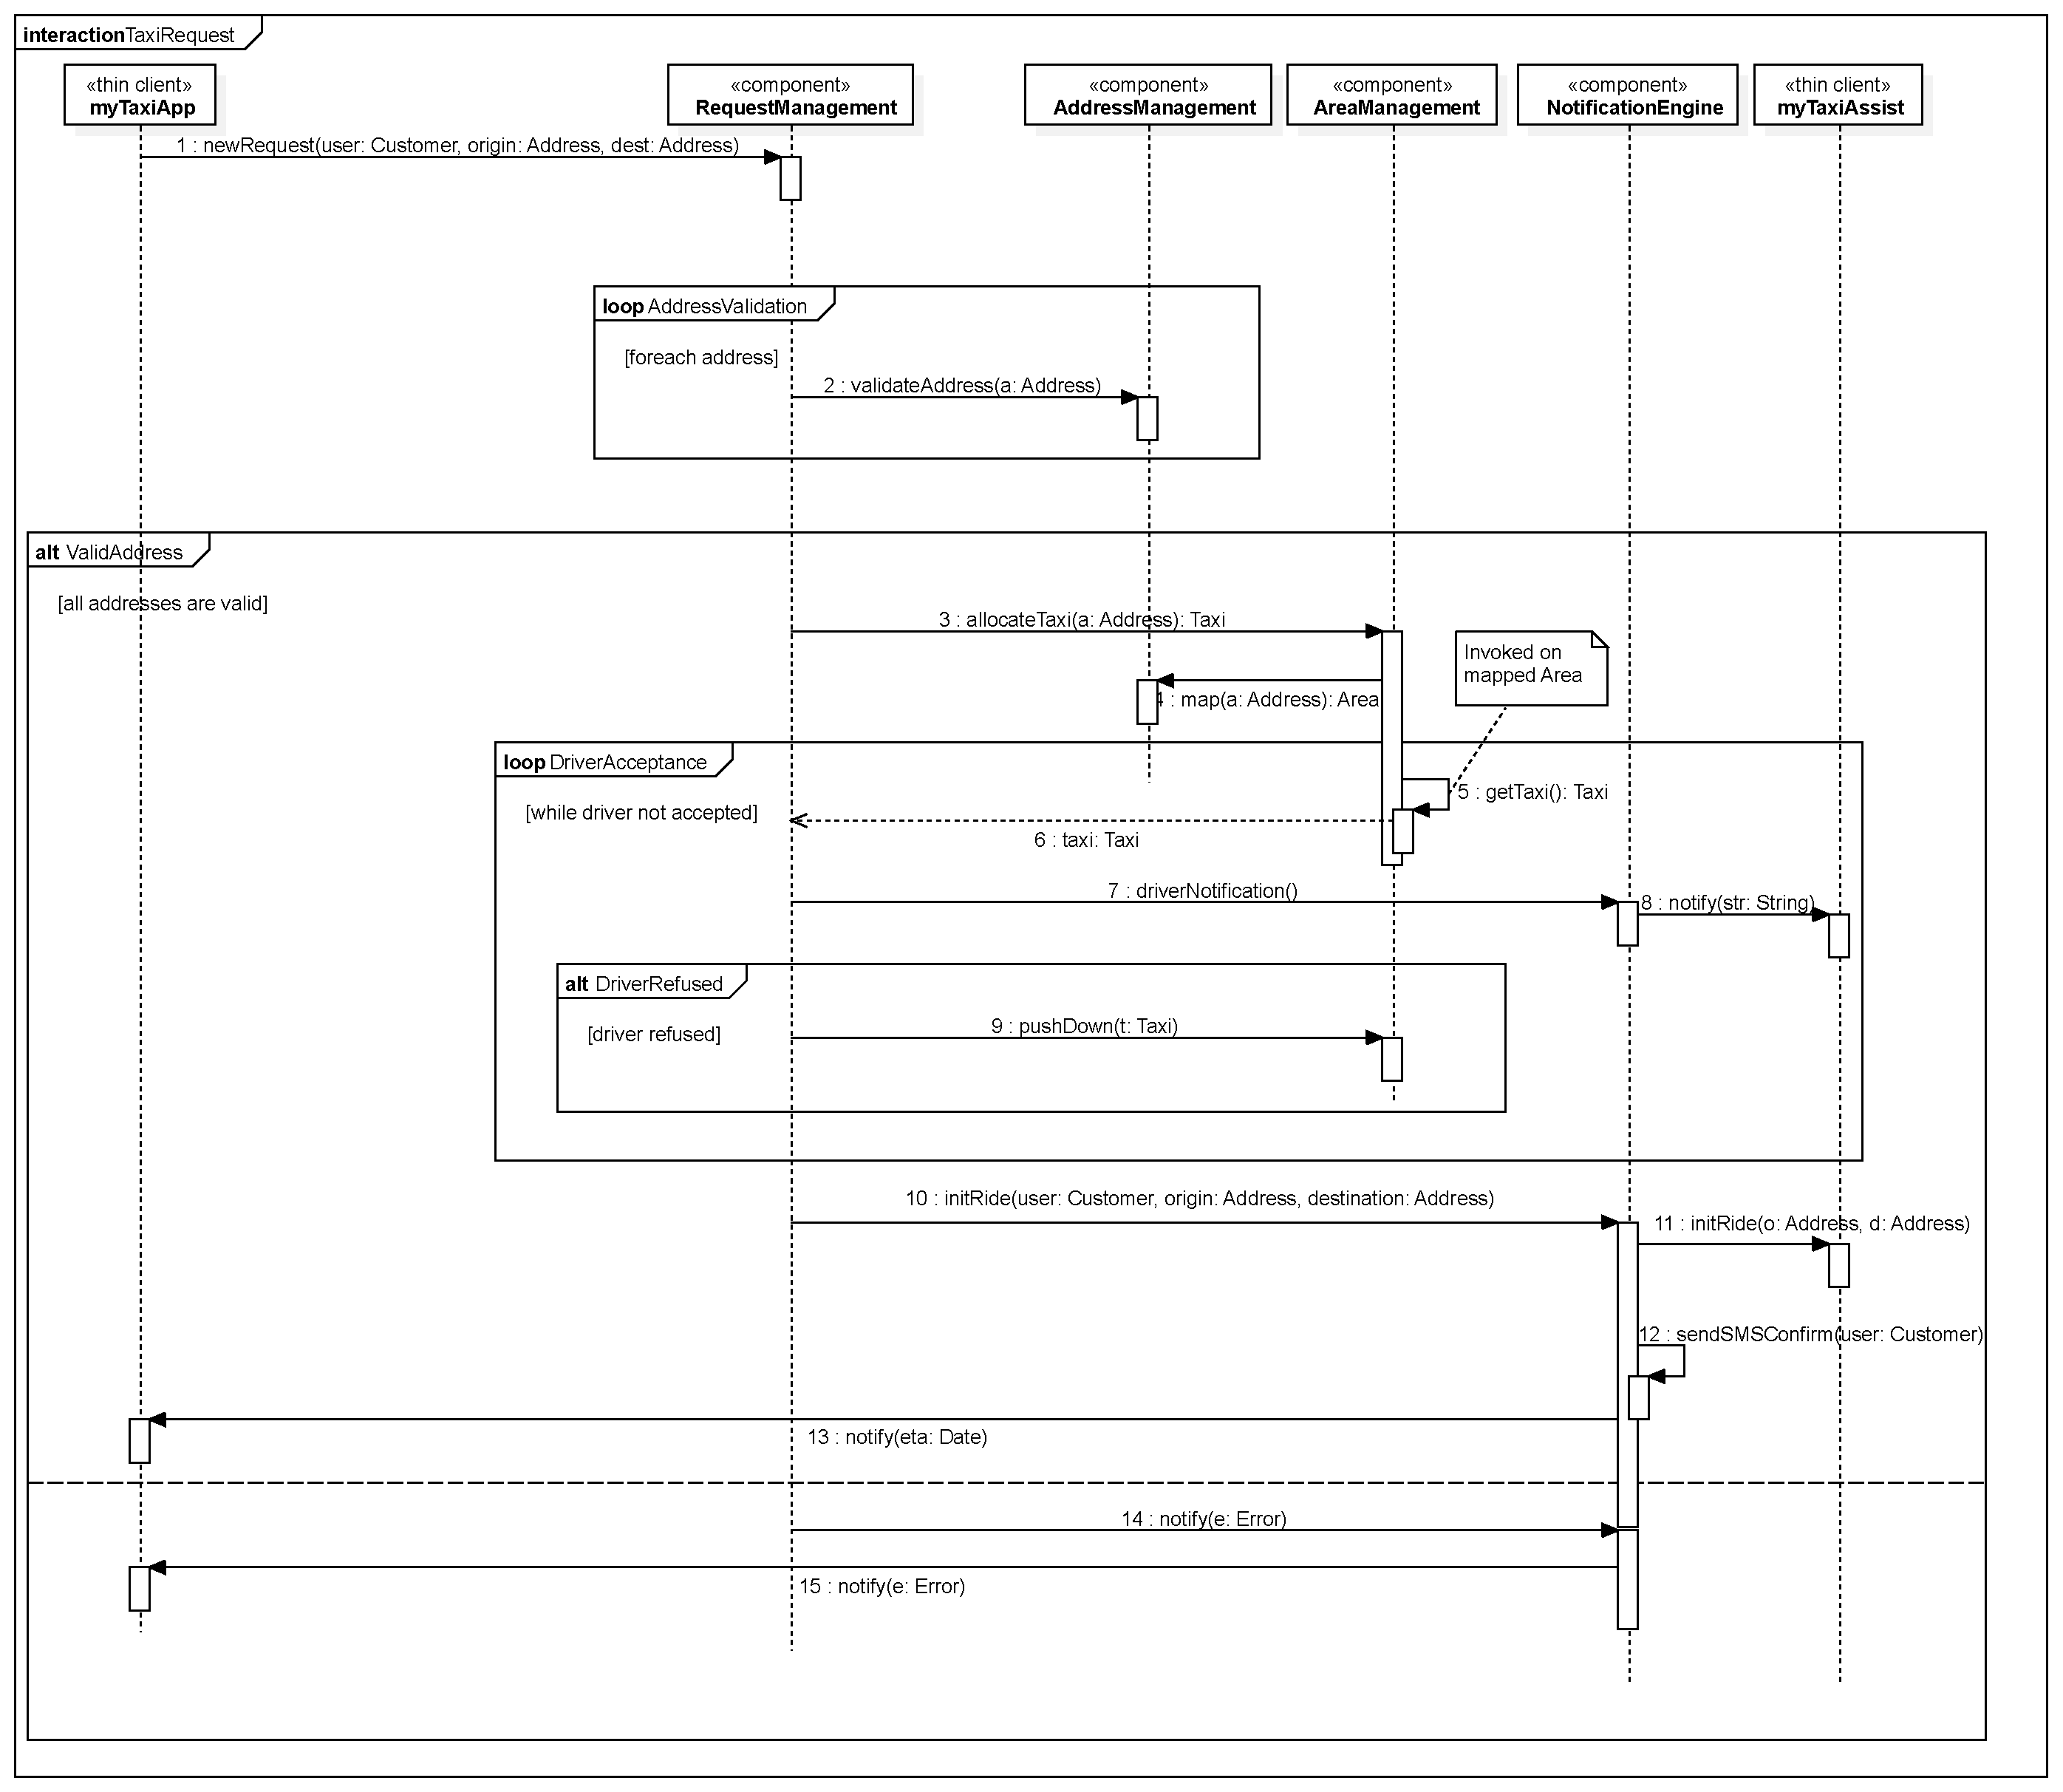
\includegraphics[width=\textwidth]{img/Sequence__Collaboration1__Interaction1__TaxiRequest_2}%
	\caption{Taxi request sequence diagram.}\label{fig:reqSequence}%
\end{figure*}

\clearpage

\begin{figure*}%
	\centering%
	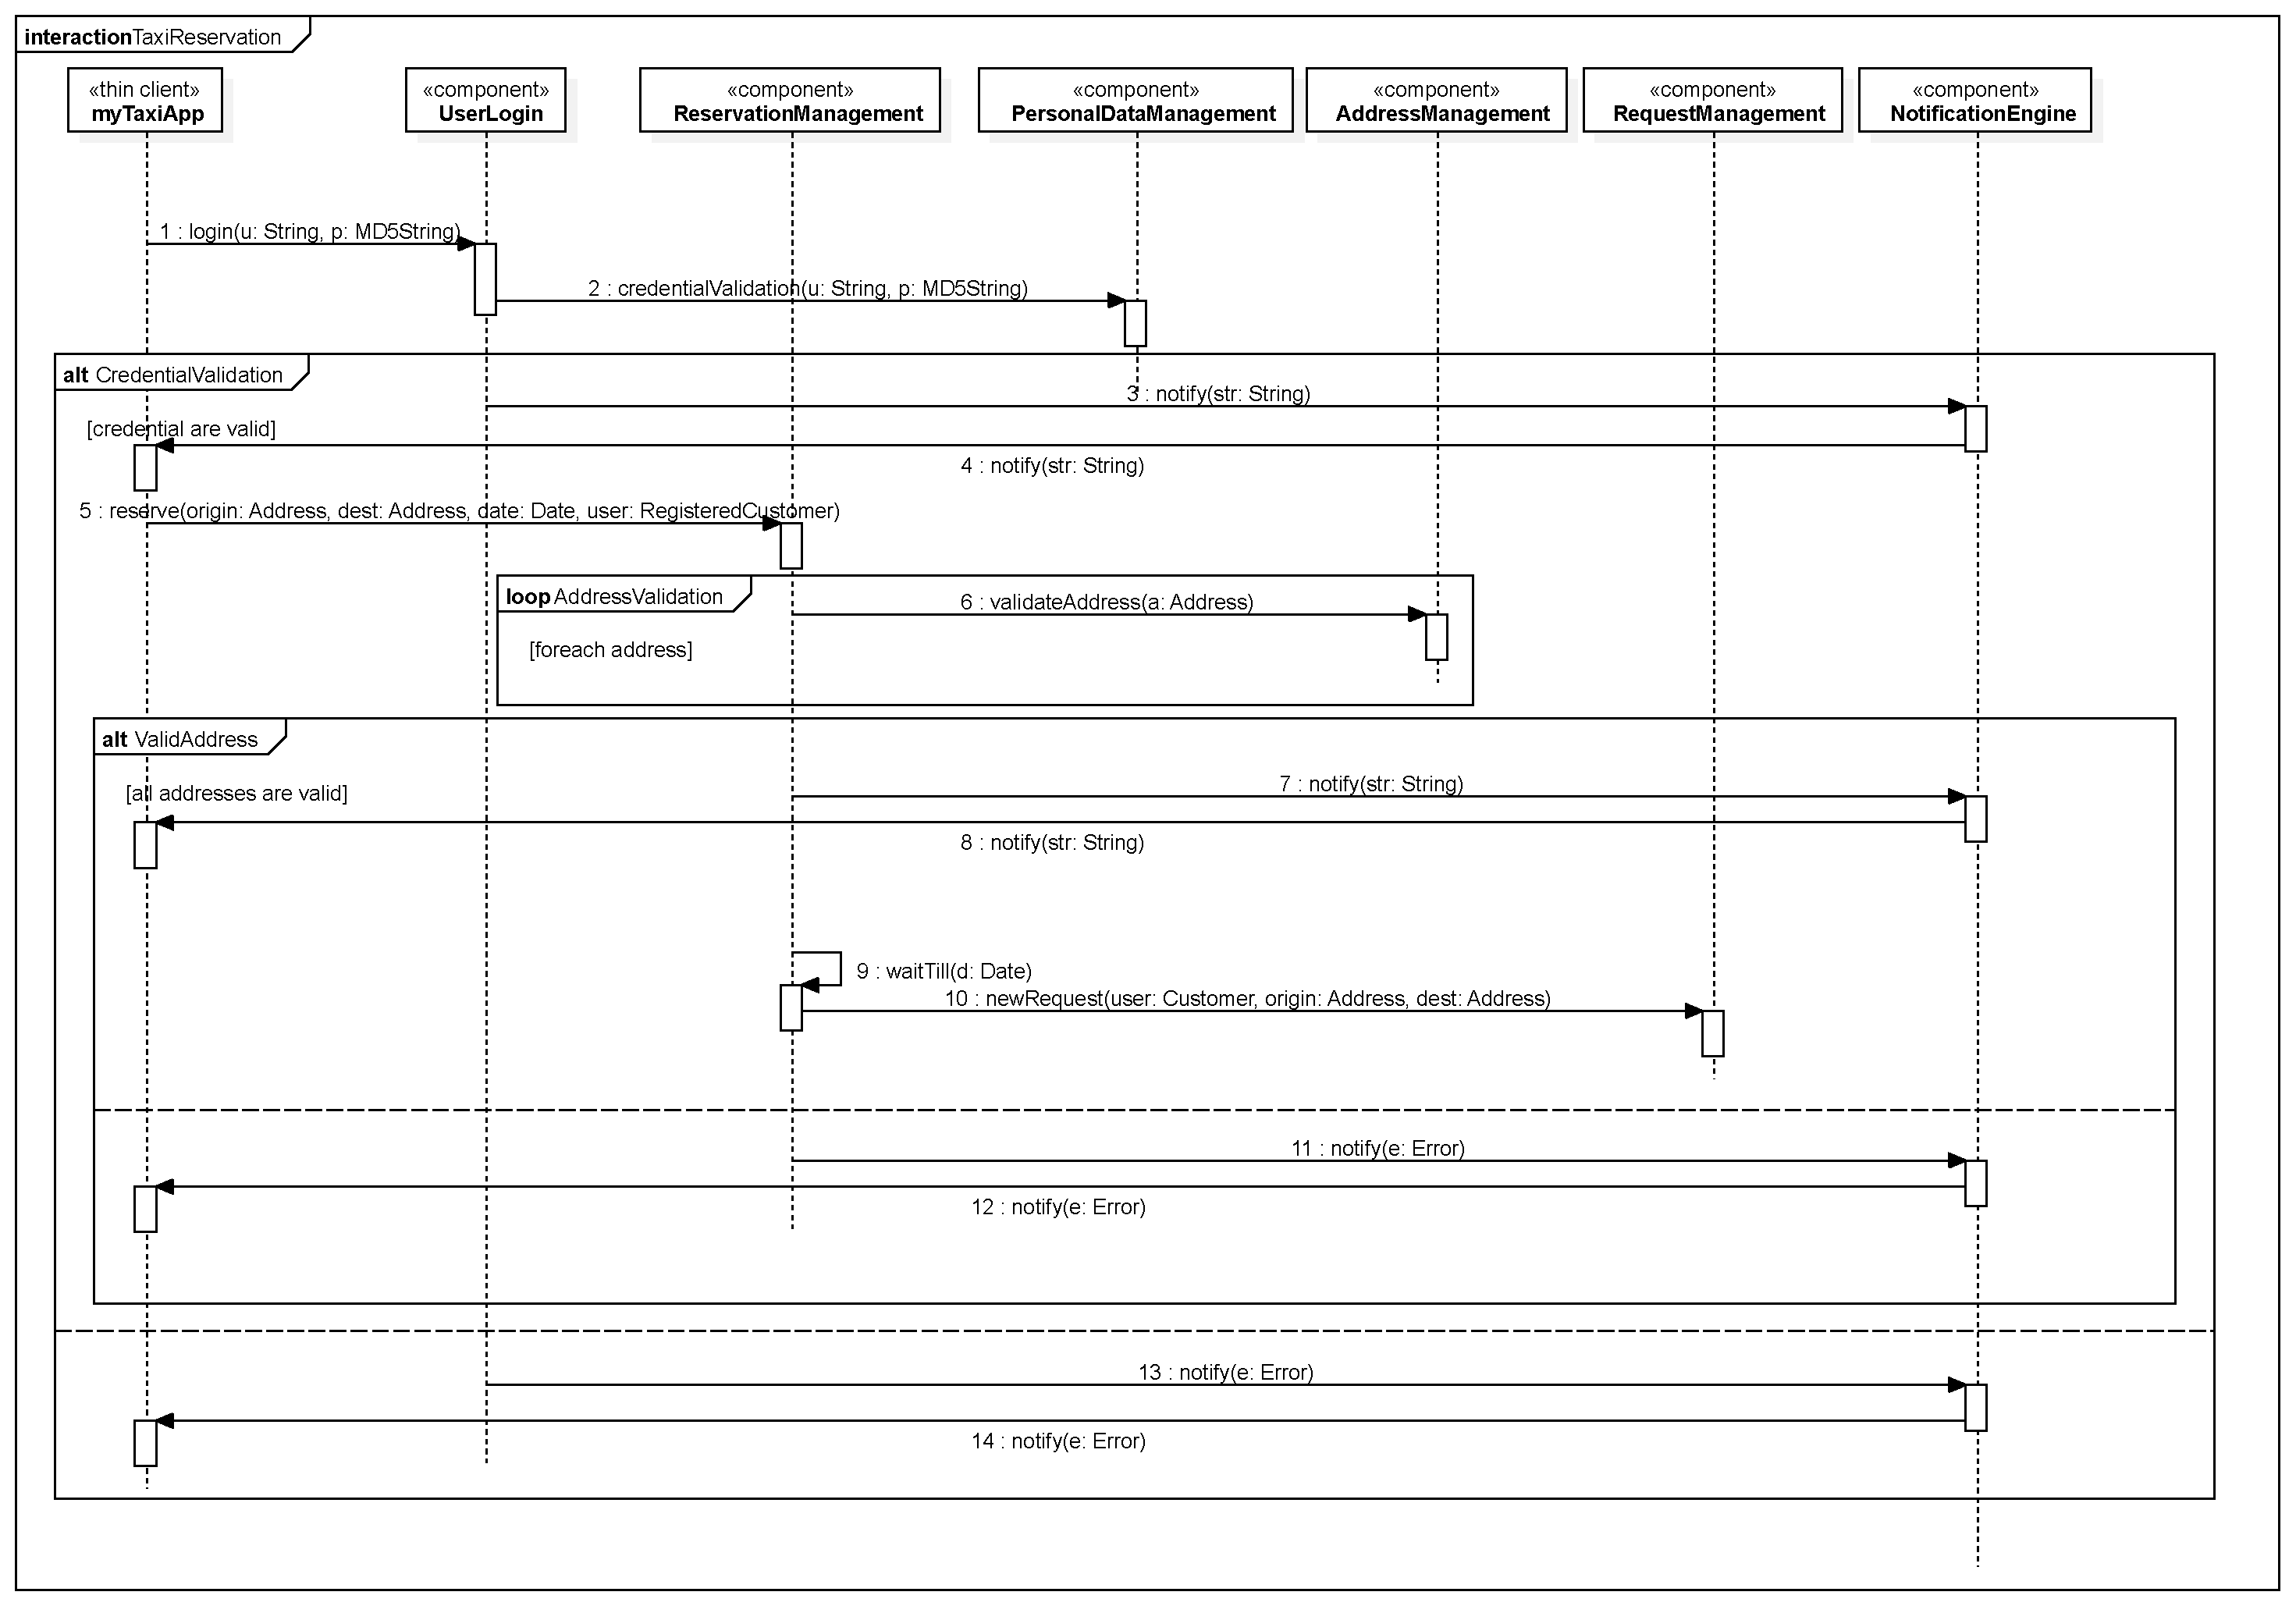
\includegraphics[width=\textwidth]{img/Sequence__Collaboration2__Interaction1__TaxiReservation_3}%
	\caption{Taxi reservation sequence diagram.}\label{fig:resSequence}%
\end{figure*}

Notice that the taxi reservation sequence diagram exploits the request procedure to complete, on the basis of what is stated in \cref{foot:reservConversion} on \cpageref{foot:reservConversion}.

Now, to complete our extensive analysis on myTaxiService ecosystem, we introduce here a runtime view of the system, by means of a \mbox{UML-like} diagram\footnote{Notice that no UML standard is defined to represent a runtime view. Nevertheless, we will use UML elements anyway, to maintain graphical consistency.}. In this diagram we represent the instances active in the system during its operation.

In particular, we are supposing the following flow of events: \begin{enumerate}
	
	\item \texttt{cus\-tom\-er1} makes a reservation for a taxi ride (\texttt{reservation1}) through myTaxiApp;
	
	\item \texttt{res\-er\-va\-tion1} is converted into a request (\texttt{re\-quest1}), and \texttt{taxi1} is allocated;
	
	\item \texttt{cus\-tom\-er2} requests a taxi ride (\texttt{re\-quest2}) via myTaxiWeb, and \texttt{taxi1} is again allocated\protect\footnote{Time constraints compliance is intended: \texttt{re\-quest2} occurs after the completion of \texttt{res\-er\-va\-tion1}/\texttt{re\-quest1} task.}.
	
\end{enumerate}

This is obviously an ideal and simplified world, which nevertheless should make clear how the system actually works. 

Some of the links between instances have been omitted, to preserve readability (for example, \texttt{res\-er\-va\-tion1} and \texttt{re\-quest1} should be both linked to \texttt{cus\-tom\-er1}, but the association was omitted, since trivial, as the request is automatically created as a result of the reservation).

\begin{figure*}%
	\centering%
	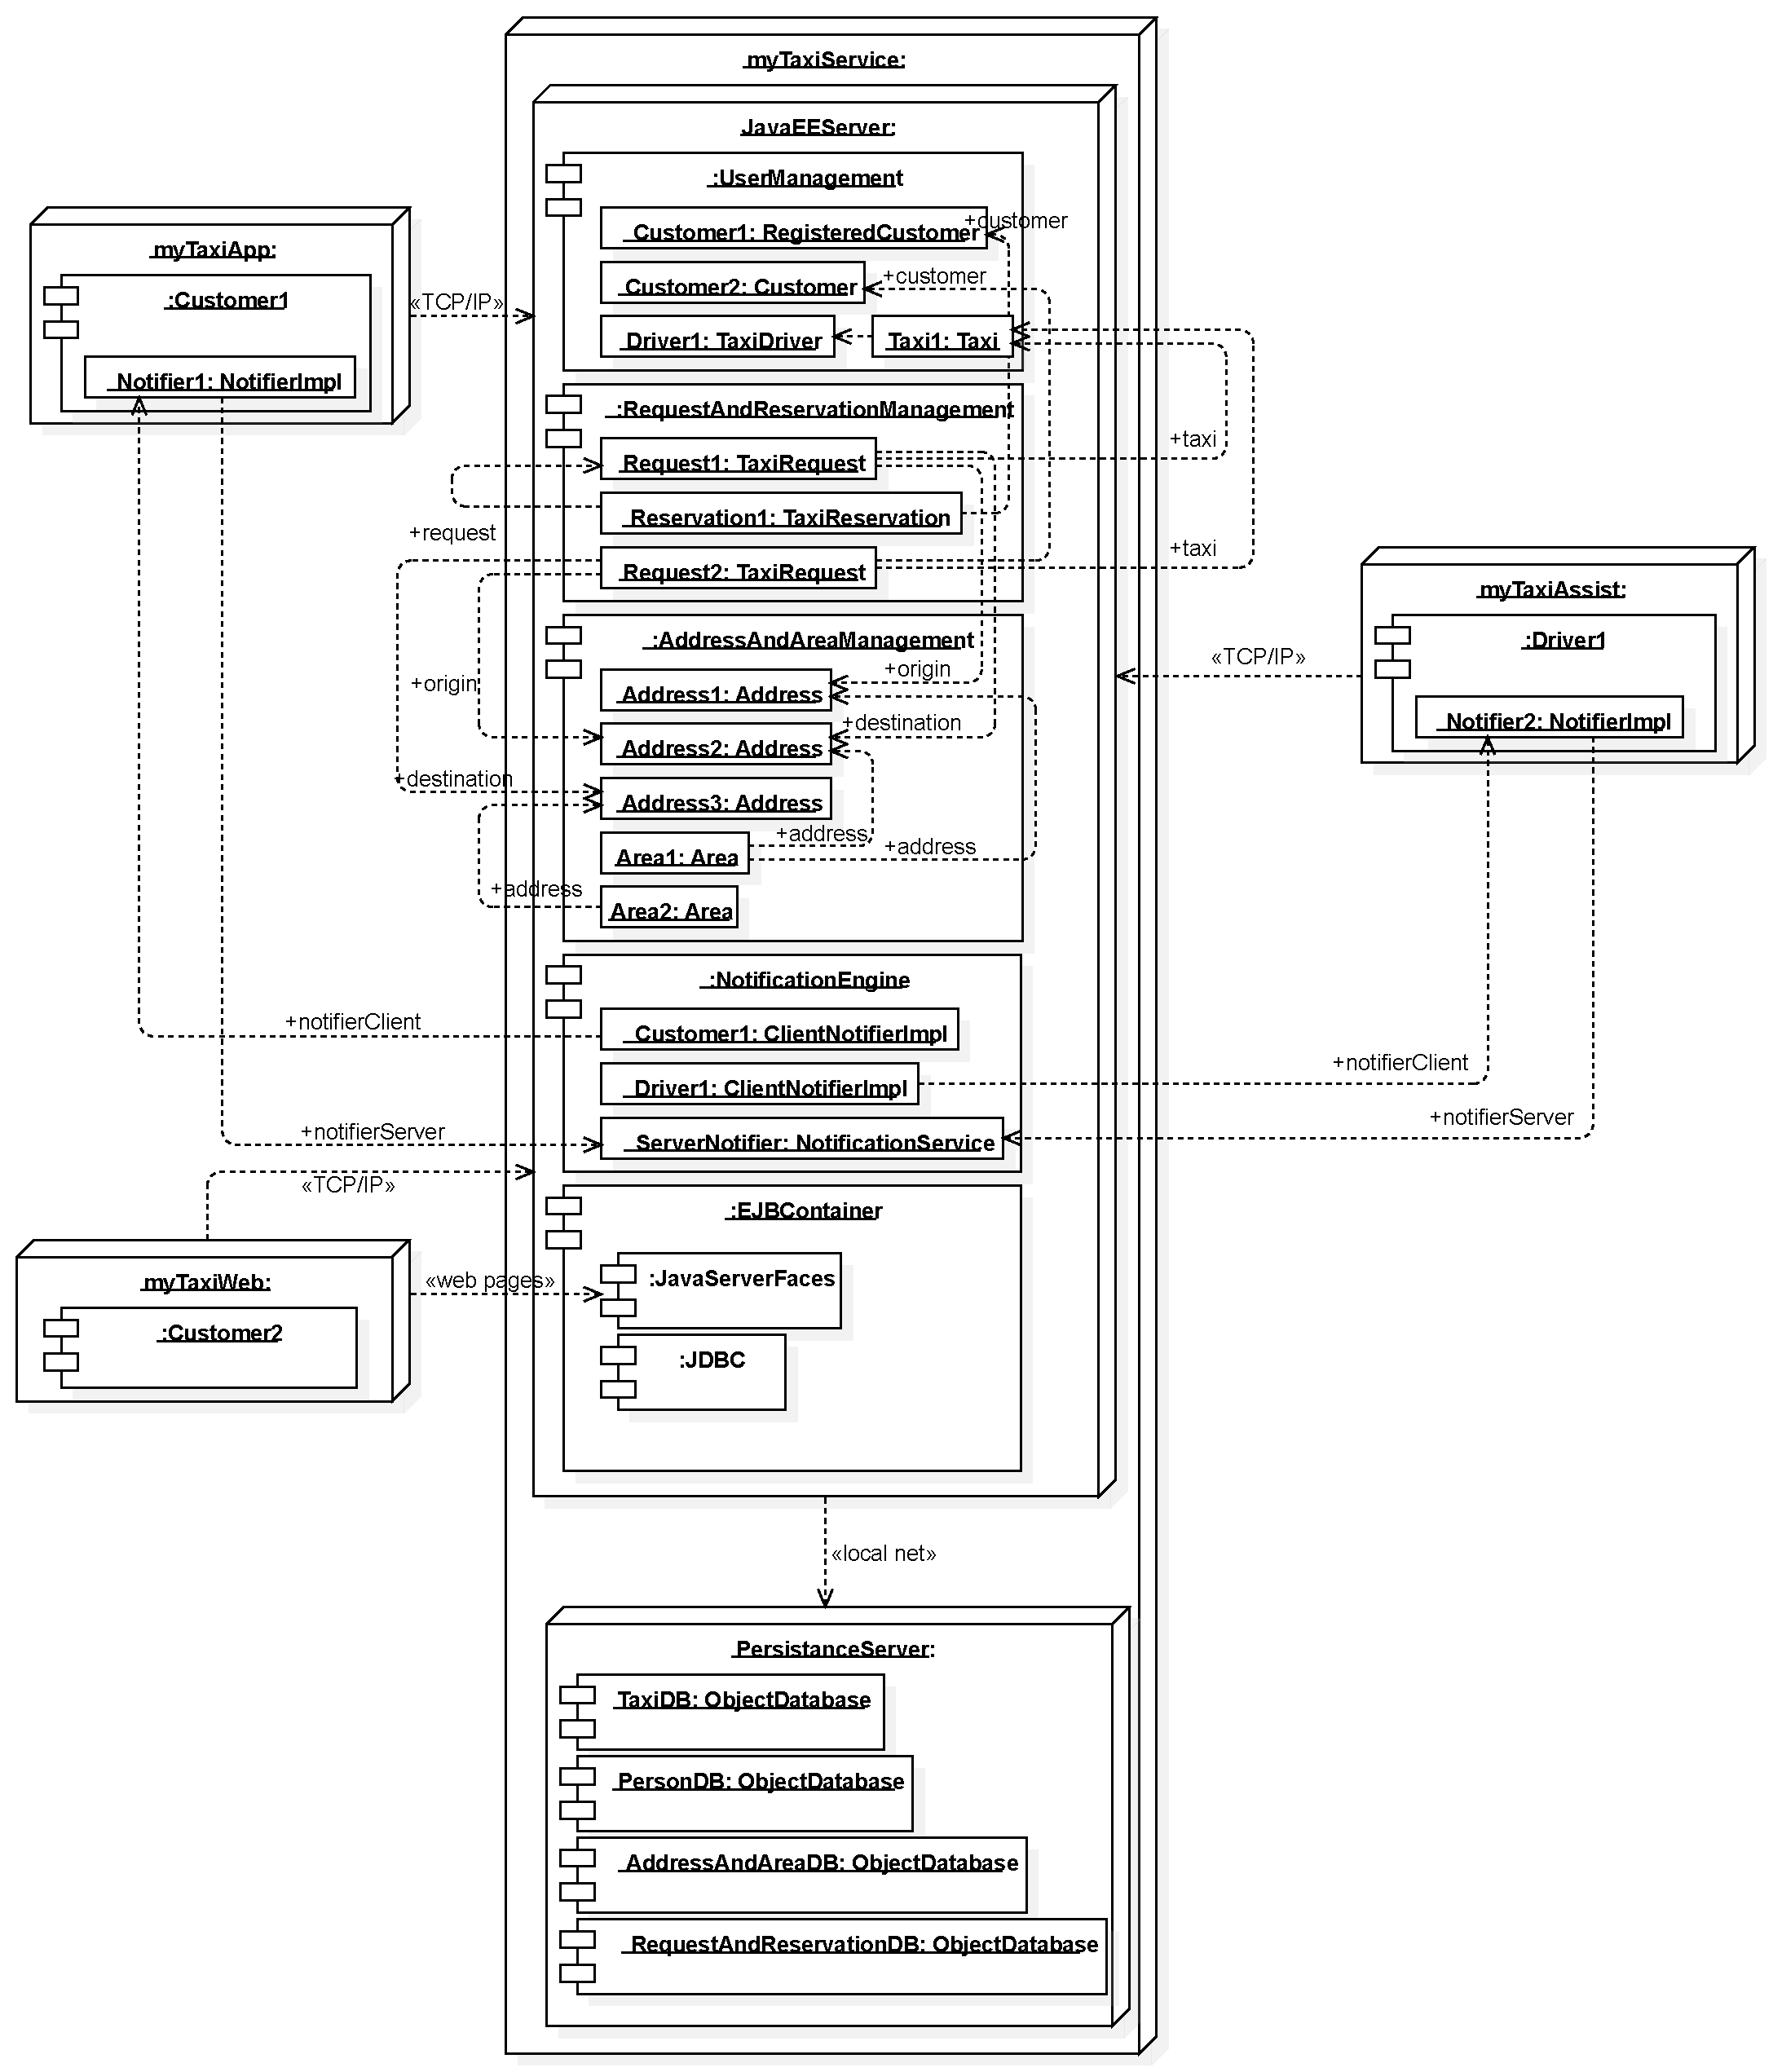
\includegraphics[width=\textwidth]{img/Runtime__RuntimeView_5}%
	\caption{Runtime view.}\label{fig:runtime}%
\end{figure*}


\clearpage


\section{Selected architectural styles and patterns}\label{sec:styles}


%Name MVC (Model-View-Controller)
%
%Description Separates presentation and interaction from the system data. The system is structured into three logical components that interact with each other. The Model component manages the system data and associated operations on that data. The View component defines and manages how the data is presented to the user. The Controller component manages user interaction (e.g., key presses, mouse clicks, etc.) and passes these interactions to the View and the Model. See Figure 6.3.
%
%Example Figure 6.4 shows the architecture of a web-based application system organized using the MVC pattern.
%
%When used Used when there are multiple ways to view and interact with data. Also used when the future requirements for interaction and presentation of data are unknown.
%
%Advantages Allows the data to change independently of its representation and vice versa. Supports presentation of the same data in different ways with changes made in one representation shown in all of them.
%
%Disadvantages Can involve additional code and code complexity when the data model and interactions are simple.


\lipsum[1-2]

\begin{figure}%
	\centering%
	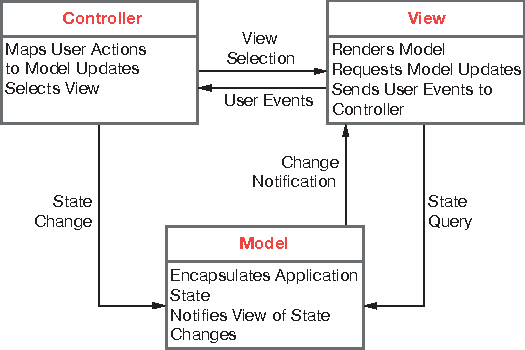
\includegraphics{img/sommMVC}%
	\caption{MVC.}
\end{figure}

%\begin{figure}%
%	\centering%
%	\includegraphics{img/sommMVCweb}%
%	\caption{MVC web.}
%\end{figure}







